\section{Design}
This chapter is about the design of the TreeWatch project. The design part is necessary to give the customer an idea of what the application will look like and so that the customer is able to give feedback. The design also gives the group members an idea of what the application should look like when it is finished. This way the group members can work towards a visual goal.

First the user should sign in, so that data is only visible to an authenticated user, as can be seen in figure \ref{signInScreen}. \\
The main goal of the application is to show all the fields on a map, with overlays of certain data. This is visualized in figure \ref{mapScreen} to figure \ref{overlayScreen}. \\
Fleuren asked to have what they call "What are you coming to do here" as part of the application. As soon as an user enters a field the application will show a screen with the question "What are you coming to do" as seen in figure \ref{comingToDoScreen}. \\
Finally there are three more screens, namely the to do list in figure \ref{toDoScreen}, the history of tasks screen in figure \ref{historyScreen} and lastly the settings screen in figure \ref{settingsScreen}.

\begin{figure}[ht]
	\minipage{0.5\textwidth}
	\centering
	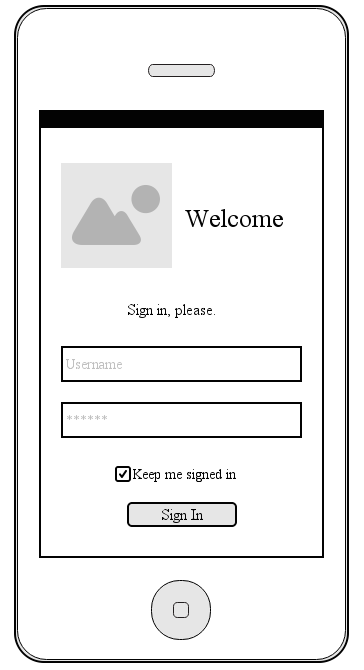
\includegraphics[width=\linewidth, height=0.4\textheight, keepaspectratio=true]{SignInScreen.png}
	\caption{Sign in screen}\label{signInScreen}
	\endminipage\hfill
	\minipage{0.5\textwidth}
	\centering
	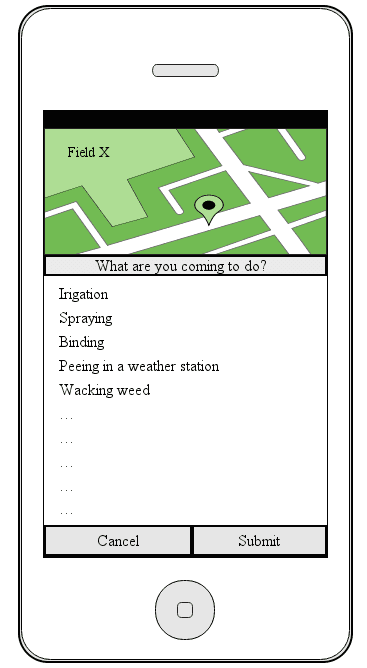
\includegraphics[width=\linewidth, height=0.4\textheight, keepaspectratio=true]{NotificationComingToDoScreen.png}
	\caption{What are you coming to do screen}\label{comingToDoScreen}
	\endminipage\hfill
\end{figure}

\begin{figure}[ht]
	\minipage{0.32\textwidth}
	\centering
	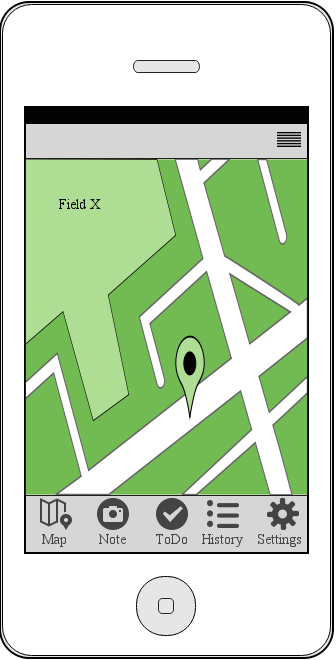
\includegraphics[width=\linewidth, height=0.4\textheight, keepaspectratio=true]{MapScreen.png}
	\caption{Default screen with the map}\label{mapScreen}
	\endminipage\hfill
	\minipage{0.32\textwidth}
	\centering
	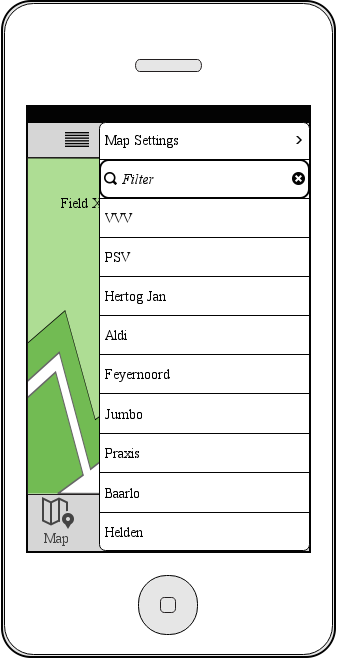
\includegraphics[width=\linewidth, height=0.4\textheight, keepaspectratio=true]{MapMenuScreen.png}
	\caption{Map screen with menu open}\label{mapMenuScreen}
	\endminipage\hfill
	\minipage{0.32\textwidth}
	\centering
	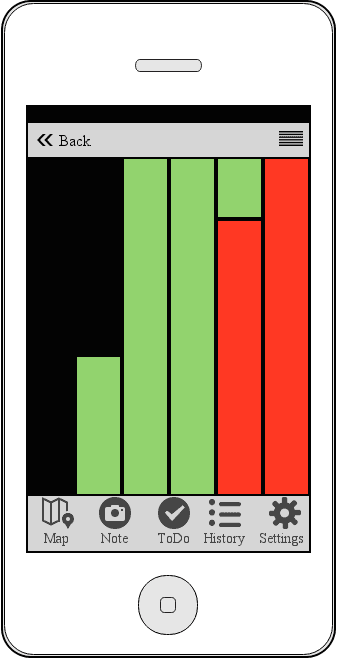
\includegraphics[width=\linewidth, height=0.4\textheight, keepaspectratio=true]{OverlayScreen.png}
	\caption{Map screen with an overlay}\label{overlayScreen}
	\endminipage\hfill
\end{figure}

\begin{figure}[ht]
	\minipage{0.32\textwidth}
	\centering
	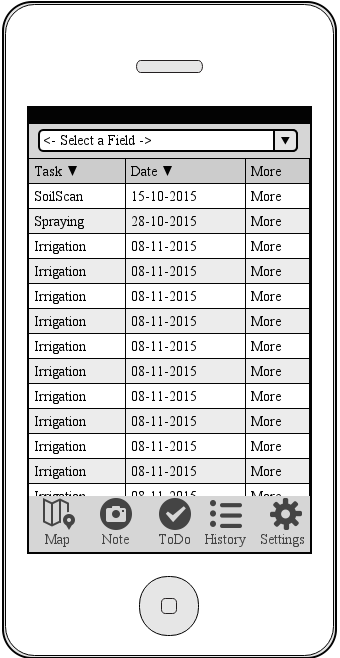
\includegraphics[width=\linewidth, height=0.4\textheight, keepaspectratio=true]{ToDoScreen.png}
	\caption{Screen where you can see to do list}\label{toDoScreen}
	\endminipage\hfill
	\minipage{0.32\textwidth}
	\centering
	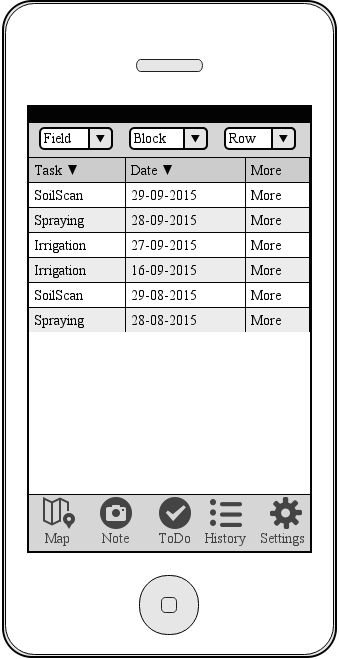
\includegraphics[width=\linewidth, height=0.4\textheight, keepaspectratio=true]{HistoryScreen.png}
	\caption{Screen with the history of tasks}\label{historyScreen}
	\endminipage\hfill
	\minipage{0.32\textwidth}
	\centering
	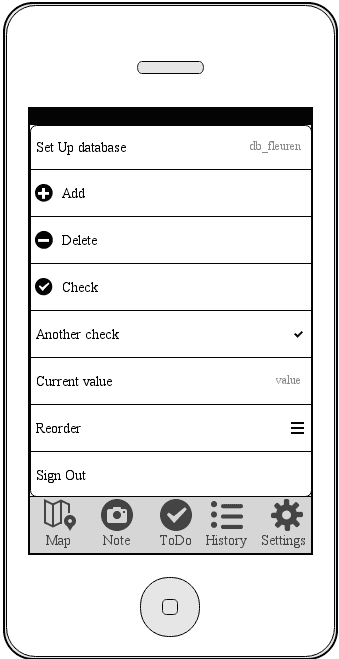
\includegraphics[width=\linewidth, height=0.4\textheight, keepaspectratio=true]{SettingsScreen.png}
	\caption{Screen where you can change settings}\label{settingsScreen}
	\endminipage\hfill
\end{figure}